
\documentclass[conference]{IEEEtran}

\usepackage{float} 
\usepackage{url}  
\usepackage{multirow}
\usepackage{caption}
\usepackage{subcaption}
\usepackage{booktabs}
\usepackage{cite}
\pagestyle{plain}
\usepackage{amsmath}
\usepackage{float}
\usepackage{tikz}
\usetikzlibrary{shapes.geometric, arrows, positioning}
\usepackage{placeins}
\usepackage{comment}
\usepackage{tabularx}
\ifCLASSINFOpdf
  \usepackage[pdftex]{graphicx}
\fi

\hyphenation{op-tical net-works semi-conduc-tor}

\begin{document}


\title{Exploring financial sentiment analysis with the Financial Phrasebank dataset}

\author{\IEEEauthorblockN{\\ Hugo Veríssimo}
\IEEEauthorblockA{Complements of Machine Learning 24/25\\
University of Aveiro\\
Aveiro, Portugal\\
hugoverissimo@ua.pt}
\and
\IEEEauthorblockN{\\ João Cardoso}
\IEEEauthorblockA{Complements of Machine Learning 24/25\\
University of Aveiro\\
Aveiro, Portugal\\
joaopcardoso@ua.pt}}

\maketitle
\thispagestyle{plain}

\begin{abstract}
abstratotoototot
\end{abstract}

\begin{quote}
\small
\noindent
\textbf{Keywords:} key, word, number, 1
\end{quote}

\IEEEpeerreviewmaketitle


\section{Introduction}

With the ever increasing volume of information created and distributed by the minute, it is more important than ever to have access to fast and reliable analysis of any information we may come across. Especially with the democratized access to financial instruments and capital markets, where individuals have the possibility to invest in virtually any company on the stock exchange, it is important to have ways to leverage against giant institutions with hundreds of financial analysts at their disposal. 

\begin{figure}[H]
    \centering
    
\includegraphics[width=0.5\linewidth]{bugs.png}
    \caption{Power to the people, colorized (circa 1917).}
    \label{fig:enter-label}
\end{figure}

Historically, financial analysis relied heavily on fundamental analysis (examining earnings, balance sheets, annual financial reports), which required extensive knowledge in the field (also the strategy that made Warren Buffett one of the richest men in the world), along with technical analysis (studying price and volume trends). Around 2010, after the 2008 global financial crisis, there was a surge in news analysis to evaluate the tone and derive investment strategies from it. Due to the lack of domain specific lexicon these analysis were falible, until the work by Loughran and McDonald was published, a financial lexicon based on 10-K forms (i.e., annual financial reports) and dictionaries. This allowed to use more sofisticated analysis rather than using the presence of negative words as a signal to sell.

Upon the launch of Twitter, information streams increased dramatically, making more and more data available for analysis. But, machine learning was not heavily used, as most data was not annotated, or there was very little data with high-quality annotations. In 2014, P. Malo \textit{et al.} published a fundamental dataset for financial sentimental analysis, that is still used, the Financial Phrasebank. It is unique, for the inclusion of important aspects as directional expressions (e.g., profits decreased), entity polarity shifts (e.g. profits may be negative if decreased), and phrase level context.

With this, machine learning models started finding their place in research, as the field of natural language processing (NLP) grew and niche fields such as financial investments found useful data. In this work we explore the Financial Phrasebank dataset, by implementing different machine learning and deep learning models to evaluate the sentiment of sentences related to financial news.

\section{State of The Art}

The field of NLP has grown drastically in the past decade, progressing from recurrent neural networks (RNN) and related models such as Long-Short Term Memory (LSTM), to the transformers-type models, large language models (LLM) and text generative models as ChatGPT. With the Financial Phrasebank the field expanded into financial analysis, with several works of relevance being published in recent years.

In the work of Araci (2019), the author developed a BERT-based model trained specifically on texts with financial data. BERT, Bidireccional Encoder Representations from Transformers, is a large language model developed by Google (2018), benefitting largely from the fact that it can "hold" in memory large chunks and in both directions, simultaneously. The fact that it is built on the Transformer encoder architecture, it can weigh the importance of different words in a sentence by using a self-attention. The model is pre-trained  on large unlabelled corpora (e.g., Wikipedia, BookCorpus), and can be fine-tuned for specific purposes. In this work, the end model was trained on  domain specific corpus such as TRC2-financial data and financial specific texts (over ~440 000 sentences), and then fine tuned with the Financial Phrasebank. The model achieved an accuracy of 97 \% on the Financial Phrasebank dataset with 100 \% agreement, but 86 \% and 85 \% respectively on the dataset with all levels of agreement (the agreement will be further detailed in the Methodology section). Later on the model was further improved by Sun \textit{et al.} (2025), EnhancedFinSentiBERT, by including dictionary embeddings, expanded corpus that deversified the pre-training stage drastically, and a novel neutral sentiment module, that further enhanced the distinction between neutral and weak sentiments, resulting in improved accuracy (89 \%) and F1-score (88 \%). The pre-training stage benefited from the large diversity of the corpus, going from a few million tokens to 2.4 B tokens with the latest version. 
In a similar direction, but at the fine tuning level, Atsiwo (2024) improved the data used in fine tuning, considering that most datasets have relatively short sentences ($<$ 100 tokens), failing to leverage the full context window  of LLMs like BERT (512 tokens). This was achieved by augmenting  the training data with synthetic sentences generated by GPT-4, with accuracy of 89 \% and F1-score of 88 \% for 50 \% agreement dataset. 

GPT has been used with different purposes, as in the work by Zhou \textit{et al.} (2023), where GPT-3.5Turbo was used for zero-shot sentiment classification. However, it performed worse than finely tuned models (accuracy of 75 \% and F1-score of 74 \%).

The BERT model was revisited by different researchers, but a new iteration from Facebook AI was proposed (2019) named RoBERTa (Robustly Optimized BERT Approach) was developed, that used a signficantly larger corpus for training (10x larger), and a dynamic masking technique during training, that allowed the model to learn new contextual relations while using the same sentences, making it more robust. This model was used as BERT to develop financial models, where the work Choe \textit{et al.} (2023) is worth mentioning, where a large corpus of financial texts were fed to the model for training, from a range of sources (e.g., Reuters, SEC fillings, EIA). The model (FiLM, Financial Language Model) benefited from the diversity of training data, rather than simply focusing on fine tuning with highly curated data, showing improved generalization and better metrics than FinBERT and RoBERTa (accuracy 88 \%, F1-score 87 \%). These models are improving substantially over the years, but it is different to put them to test against a controlled dataset from using them in real life, and the variety included as consequence. Competitions such as FinNLP help drive research in this field, by posing ever more diversified test sets, aiming to improve the robustness of models, and the solutions developed by the researchers.


\section{Methodology}

To address the problem of sentiment classification in sentences related to financial investment, we set up a pipeline for training and testing using the Financial PhraseBank for three types of models, where the best was further explored and tuned for different tests. The dataset and setup is detailed in the following sections.

\subsection{Dataset}

% Acho que não precisamos disto aqui https://huggingface.co/datasets/takala/financial\_phrasebank
The Financial PhraseBank is a widely used benchmark dataset for financial sentiment analysis. It consists of roughly 4,840 English sentences (mostly news headlines or short statements) about companies, drawn from financial news articles and press releases. Each sentence is labeled with one of three sentiment classes – positive, negative, or neutral – representing the sentence’s sentiment from the perspective of an investor \cite{dataset, malo2013gooddebtbaddebt}.

\begin{table}[H]
\centering
\caption{Financial PhraseBank distribution. Four possible sets within the dataset, depending on how many financial experts agreed with the attributed label. The dataset with 50 \% agreement corresponds to the entire dataset.}

\label{agreement_datasets}
\begin{tabular}{lcccc}
\toprule
\textbf{Sentiment} & \multicolumn{4}{c}{\textbf{Agreement}} \\
\cmidrule(lr){2-5}
 & \textbf{50\%} & \textbf{66\%} & \textbf{75\%} & \textbf{All} \\
\midrule
Negative & 604 & 514 & 420 & 303 \\
Neutral & 2879 & 2535 & 2146 & 1391 \\
Positive & 1363 & 1168 & 887 & 570 \\
\midrule
\textbf{Total} & 4846 & 4217 & 3453 & 2264 \\
\bottomrule
\end{tabular}
\end{table}

The dataset was labeled by 16 finance professionals, each responsible for labelling a subset of sentences. Each sentence was labelled by 5-8 annotators, and the resulting agreement score was a result of the fraction of annotators that labelled the sentence in the same manner. This resulted in 4 different subsets, where 50 \% agreement corresponds to the entire dataset, with the dataset size decreasing as the level of agreement increased. It is important to mention that the agreement level corresponds to the least allowed, so the 50 \% agreement level dataset contains the other subsets. The dataset sizes and class proportion can be consulted in Table \ref{agreement_datasets}, along with sample sentences and the attributed sentiment classification in Table \ref{tab:fpb_examples}.

This subset strategy allows researchers to find a balance between the amount and the quality of data, representing a common trade-off in the field of machine learning.

%o dataset foi anotado (labels) por 16 anotadores com background em economia/finanças, sendo que cada anotou um subset de frases. cada instância foi anotada por 5-8 anotadores independentes, levando então à criação de 5 sub datasets tendo em conta o nível de concordaância entre as anotações: 50\% de agreement, 66\%, 75\%, e concordância total. a distribuição das classes juntamente com a quantidade total de instancias é apresentada na tabela \ref{agreement_datasets}. importa também referir que a cada determinada concordância é um mínimo, ou seja, por exemplo o dataset de 50\% de Agreement contem os datasets de 66\%, 75\% e total concordância.

%estes subsets permitem aos investigadores ter um equilíbrio entre quantidade de dados e qualide dos dados, representando um trade-off muito comum no espaço da aprendizagem automática (ig)

VER MAIS COISAS SOBRE OS DADOS AINDA

% exemplos de frases

\begin{table}[ht]
\centering
\caption{Example sentences from the Financial PhraseBank with annotated sentiment labels.}
\label{tab:fpb_examples}
\begin{tabular}{p{6.4cm}p{1.6cm}}
\toprule
\textbf{Sentence} & \textbf{Sentiment} \\
\midrule
According to Gran, the company has no plans to move all production to Russia, although that is where the company is growing. & Neutral \\
Componenta's net sales doubled to EUR~131m, moving to zero pre-tax profit from a EUR~7m loss. & Positive \\
In Q3 2010, net sales increased by 5.2\% to EUR~205.5mn, and operating profit by 34.9\% to EUR~23.5mn. & Positive \\
Operating profit totalled EUR~21.1mn, up from EUR~18.6mn in 2007, representing 9.7\% of net sales. & Positive \\
\bottomrule
\end{tabular}
\end{table}


Considera adicionar o nível de concordância para as frases, já que pode ser interessante perceber porque é que foi mais difícil concordarem

Unique samples from 50Agree:

% In banking , Sampo A was unchanged at 14.24 eur and Nordea rose 0.42 pct to 9.51 eur .

casos de pequenas pcts , apesar de ser subida

% Previously , the company also delivered about 70 % of the steel used in Oasis of the Seas , Allure of the Seas ' sister ship completed last year .

resultados passados


Unique samples from 66Agree:

%Basic banking activities continued as normal .

normal é bom?

%Finnish software and hardware developer Elektrobit Oyj HEL : EBG1V , or EB , said today it will temporarily lay off up to 200 people for a maximum of 90 day in Finland , aiming to achieve cost savings of EUR 1.7 million USD 2m in the second half of 2010 .

lay off, but limited time



\subsection{Exploratory Data Analysis}

Taking into consideration the different possible subsets, we selected the one with 75 \% agreement, as it is a balance between quantity and quality in the dataset, also taking into consideration the proportion between classes.

In Fig. \ref{fig:sentiment_distribution} the number of sentences per class is evidence of how imbalanced the dataset is. As a result, we had to balance the dataset by undersampling all classes to the amount of examples for the 'negative' class, the .

%tendo em conta os vários subsets dispobíveis do Financial Phrasebank, o escolhido para análise mais detalhada ao longo deste projeto foi o dataset 75Agreement, representado possivelmente o melhor equilibrio entre qualidade e quantidade, tendo em conta a qnt de instancia por classe face às restantes concordâncias.

\begin{figure}[H]
    \centering
    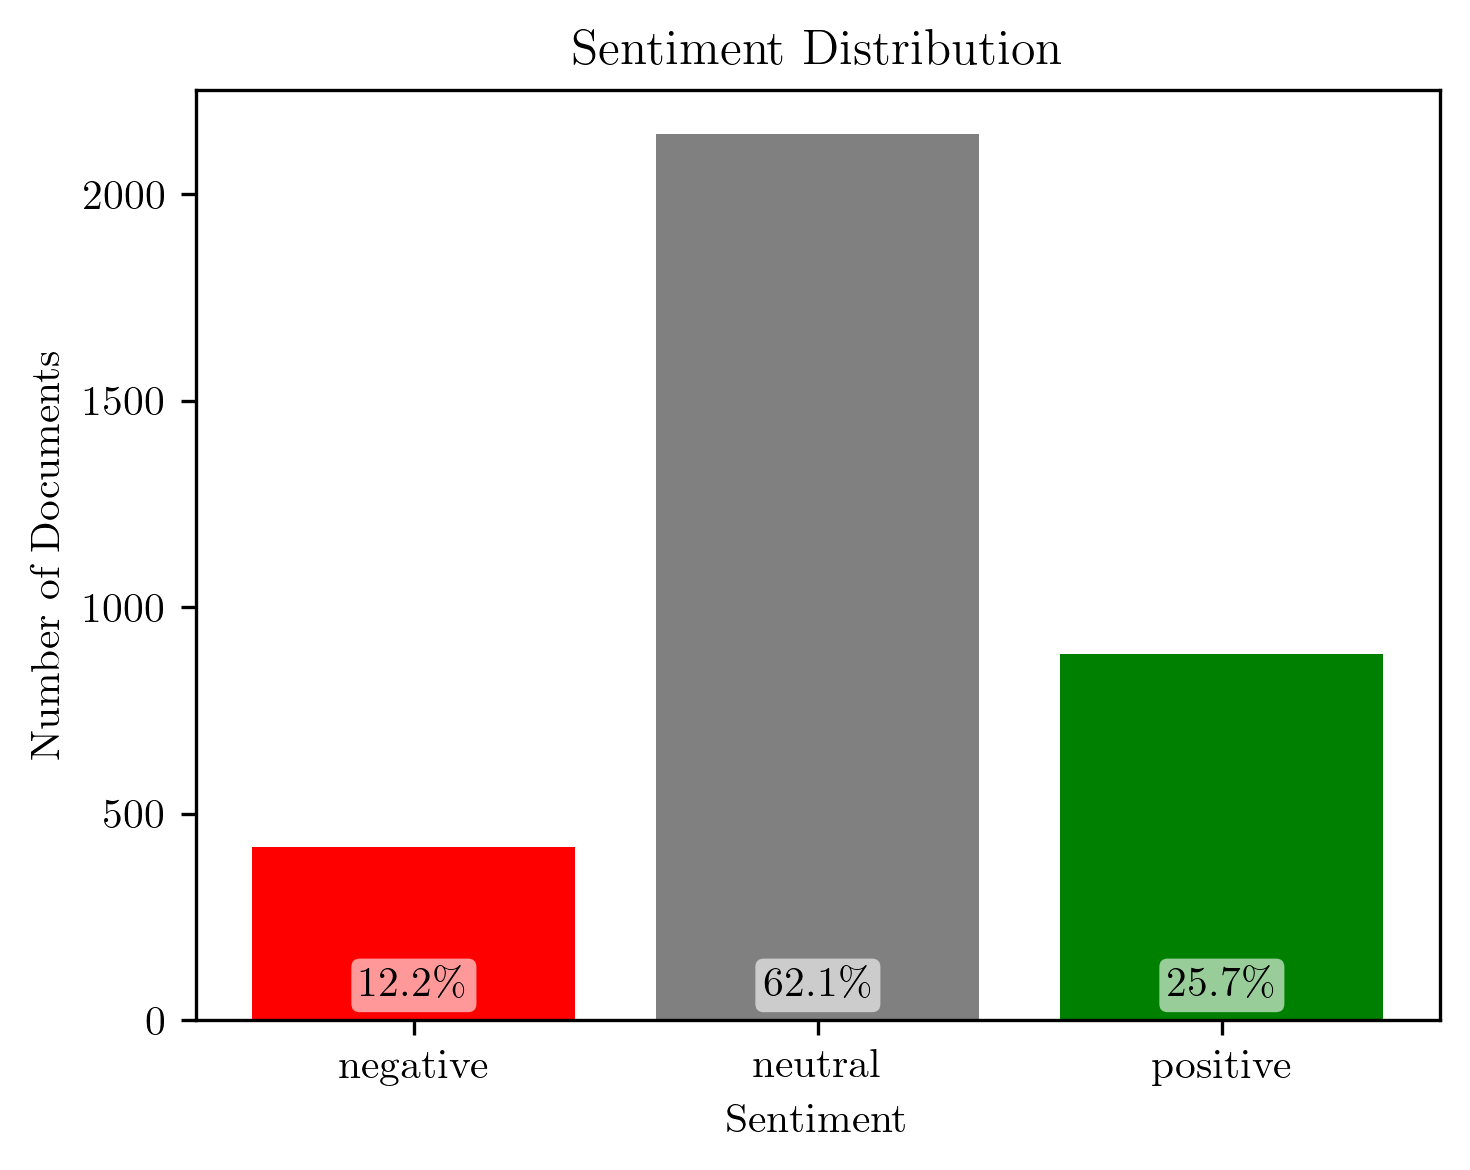
\includegraphics[width=1\linewidth]{assets/sentiment_distribution.png}
    \caption{Class distribution in the 75 \% agreement dataset.}
    \label{fig:sentiment_distribution}
\end{figure}


In cl
\begin{figure}[H]
    \centering
    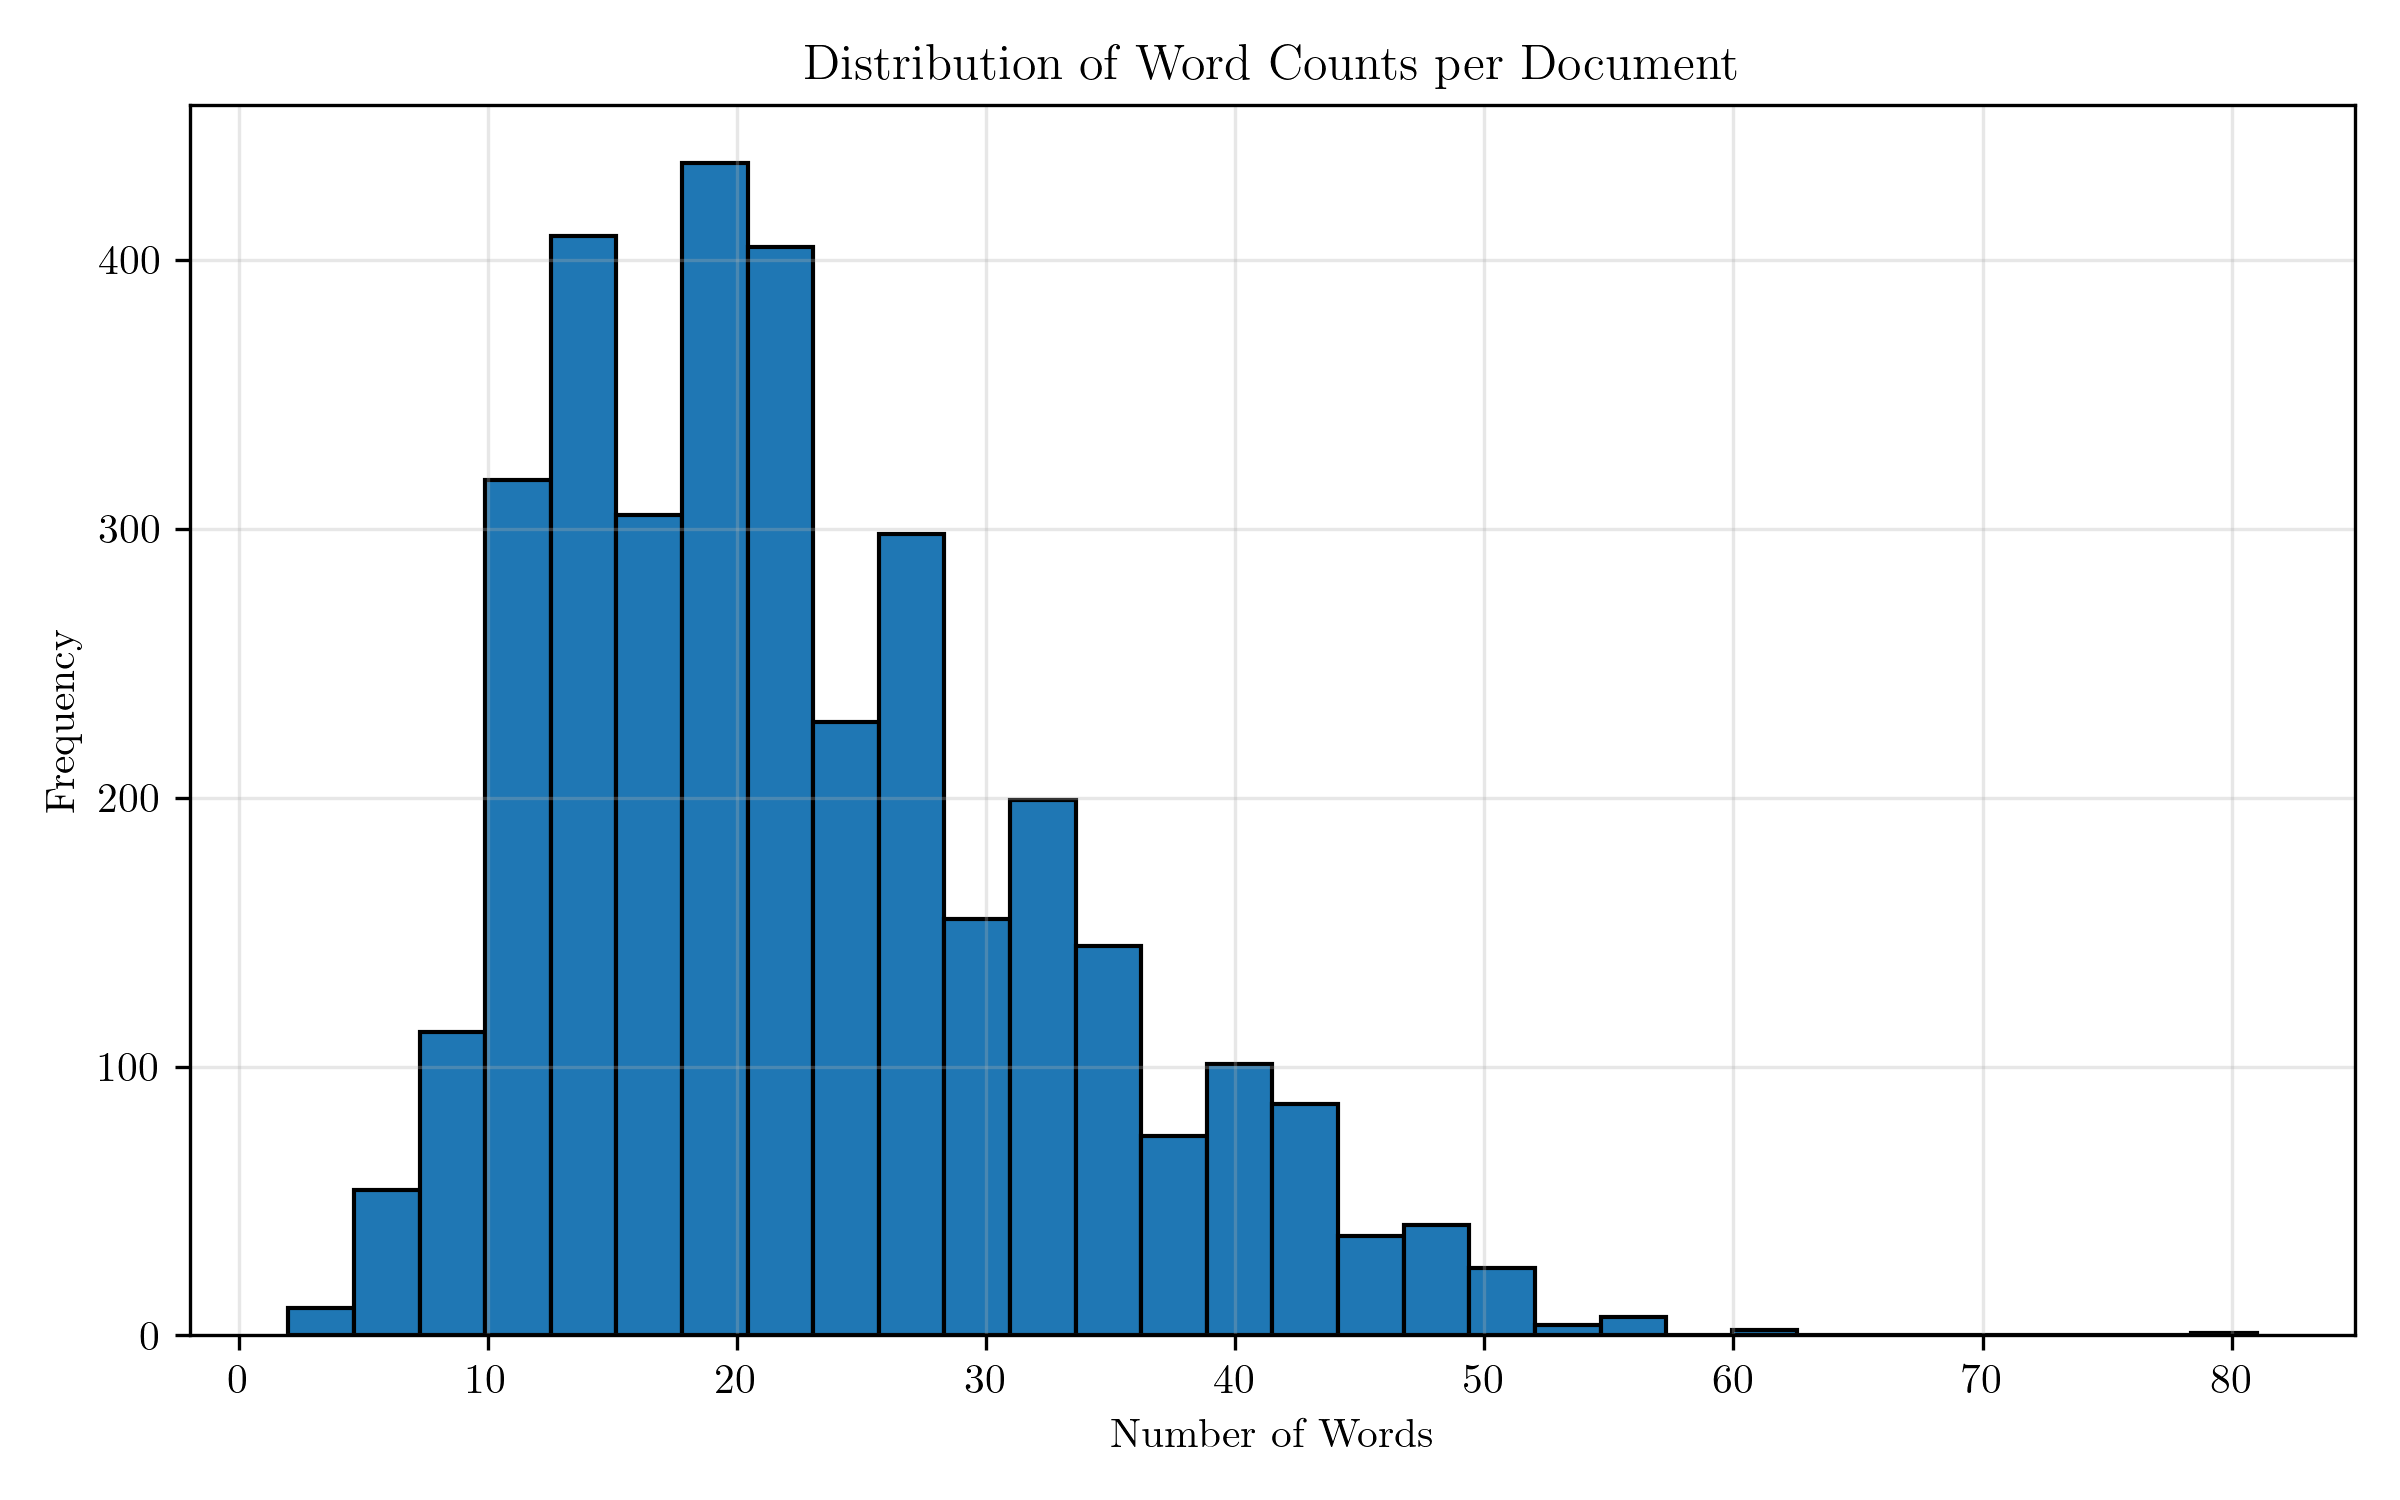
\includegraphics[width=1\linewidth]{assets/word_count_distribution.png}
    \caption{Sentence length distribution for the 75 \% agreement dataset.}
    \label{fig:word_count_distribution}
\end{figure}

este word count dist ajudou na escolha do numero de tokens a usar, o max len nos tokenizers \ref{fig:word_count_distribution}

\begin{figure}[H]
    \centering
    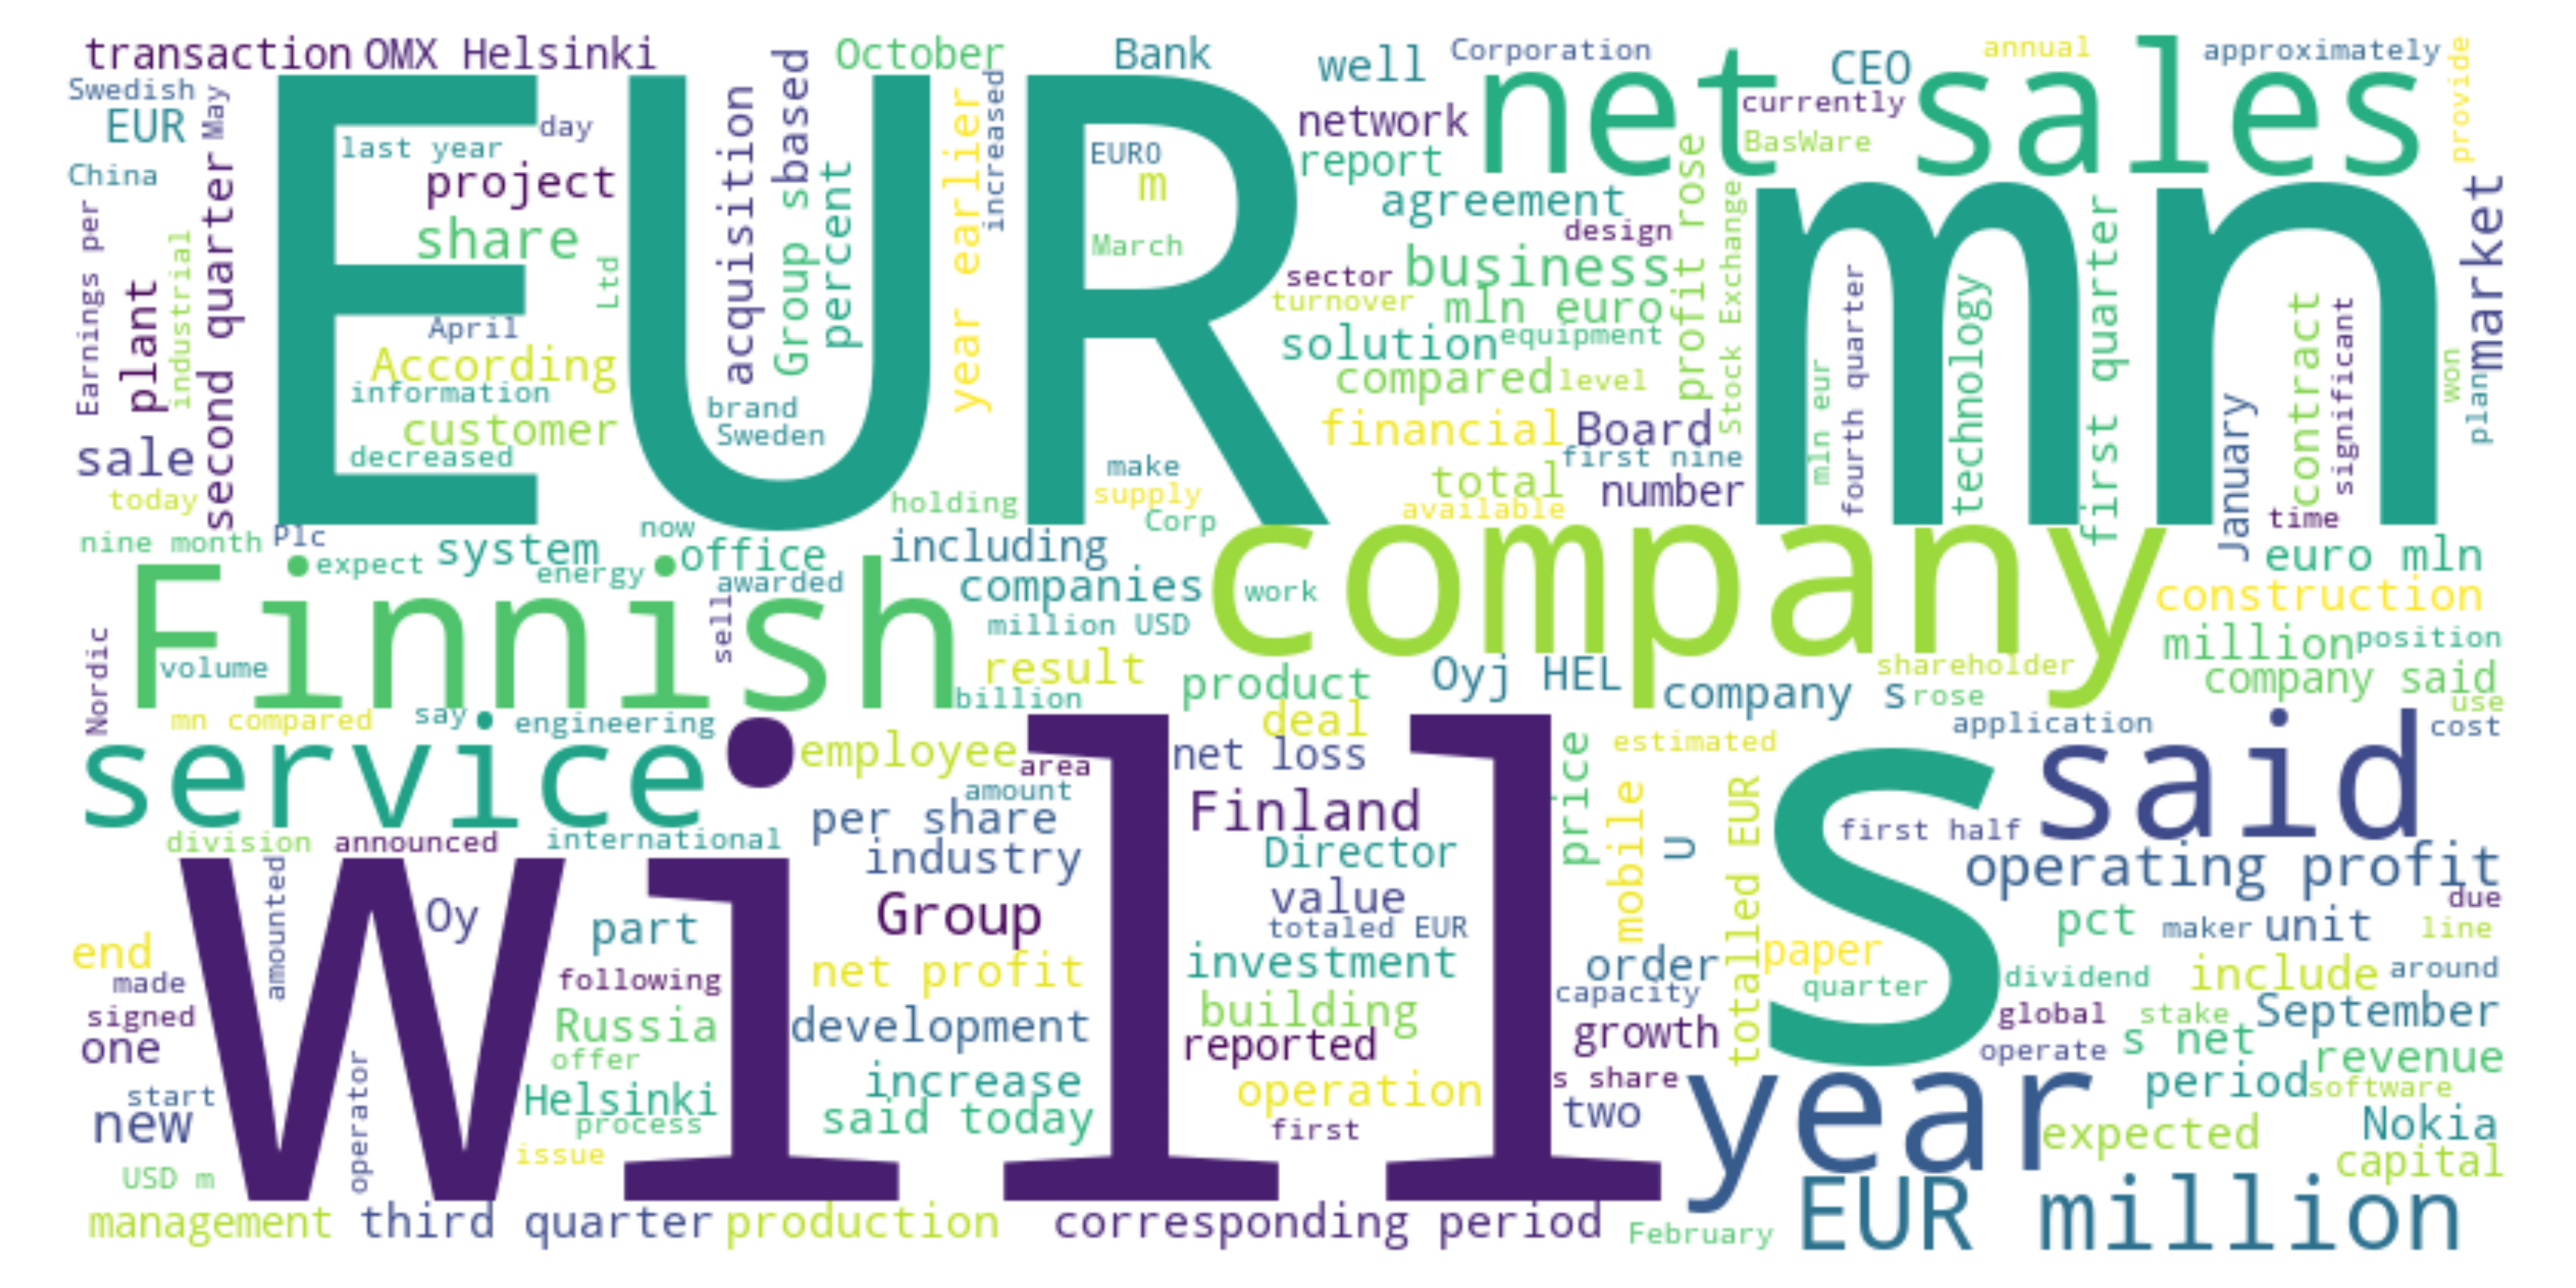
\includegraphics[width=1\linewidth]{assets/word_cloud_75agree.png}
    \caption{most common words in the sentences}
    \label{fig:word_cloud_75agree}
\end{figure}

most relevant words for class identification by checking which words appear much more in one class than others: down, decreased, profit, fell, rose


\subsection{Preprocessing}

split teste e treino (80/20) do dataset de 75 de agreement

dps tendo em conta essa porção de 20, tbm se removeu esses documentos dos restantes subsets para evitar possivel leakage (pq usamos dps os subsets na cena dos pesos, ns como queres dizer ou se faz sentido dizer aqui se quer)

o preprocessamento dos dados acabou por variar de modelo para modelo, em termos da estrura dos dados ou transofmacoes nas frases tendo por base os pre requistos dos mesmos, sendo a unica constante o balanceamento das classes nos dados de treino antes de qualquer tunning ou treino.

\subsection{HELP}

imagina, esta secção é metodologia, fará sentido dizer aqui de vez o cv validtion já q ele é usado sempre? se sim, está mesmo aqui em baixo o como ele foi feito mas tldr 5-cv escolha dos melhores hyp, re treino no conjunto de treino completo

learning curve + comparacao de metricas de teste e de treino para evitar overfitting

\section{Models ????}

sendo que o objetivo principal é ent a classificacao das frases presentes no conjunto de teste (20\% do subset do 75agree), foram exploradas três abordagens distintas focando no equilibrio de entre quantidade e qualidade dos dados

- base model

- data augmention model

- weighted model

\subsection{A. Initial benchmark}

Falar sobre os modelos que usámos para este trabalho e as suas arquitecturas, FASTTEXT, LSTM, 
FALTA METER AQUI FASTTEXT, LSTM, ...

dataset so se usou o 75agree com o split 80/20 feito inicialmente

houve fine tunning dos hyp para cada um dos modelos usando 5-fold cv para a escolha destes e depois retreino com estes hyp nos dados de treino completos

\begin{table}[H]
\centering
\caption{base model metrics across models}
\label{basemodel_models}
\begin{tabular}{lcccc}
\toprule
\textbf{Model} & \multicolumn{2}{c}{\textbf{Accuracy}} & \multicolumn{2}{c}{\textbf{F1 (weighted)}} \\
\cmidrule(lr){2-3} \cmidrule(lr){4-5}
 & \textbf{Train} & \textbf{Test} & \textbf{Train} & \textbf{Test} \\
\midrule
fastText & 0.54 & 0.65 & 0.45 & 0.58 \\
LSTM & 0.67 & 0.66 & 0.63 & 0.63 \\
BERT & 0.97 & 0.92 & 0.97 & 0.92 \\
\bottomrule
\end{tabular}
\end{table}

apesar de ainda n ter a tabela fastext < lstm < bert

lstm vai ao encontro dos resulados descritos na literatura, apesar de um pouco piores por n termos usado bi-LSTM nem ELMo, seja lá oq isso for


sendo que o bert foi o melhor, indicamos mais detalhes osbre o modelo:::

\begin{table}[H]
\centering
\caption{Hyperparameter space for ......}
\label{parameters_basebert}
\begin{tabular}{ll}
\toprule
\textbf{Hyperparameter} & \textbf{Possible Values} \\
\midrule
Epochs & $\{1,2,3,4,5\}$ \\
Learning rate & $[10^{-5}, 10^{-2}]$ \\
Weight decay & $[0, 0.5]$ \\
\bottomrule
\end{tabular}
\end{table}

best hyperameters: 

- Num train epochs: 2

- Learning rate: 0.0001

- Weight decay: 0.1

\begin{figure}[H]
    \centering
    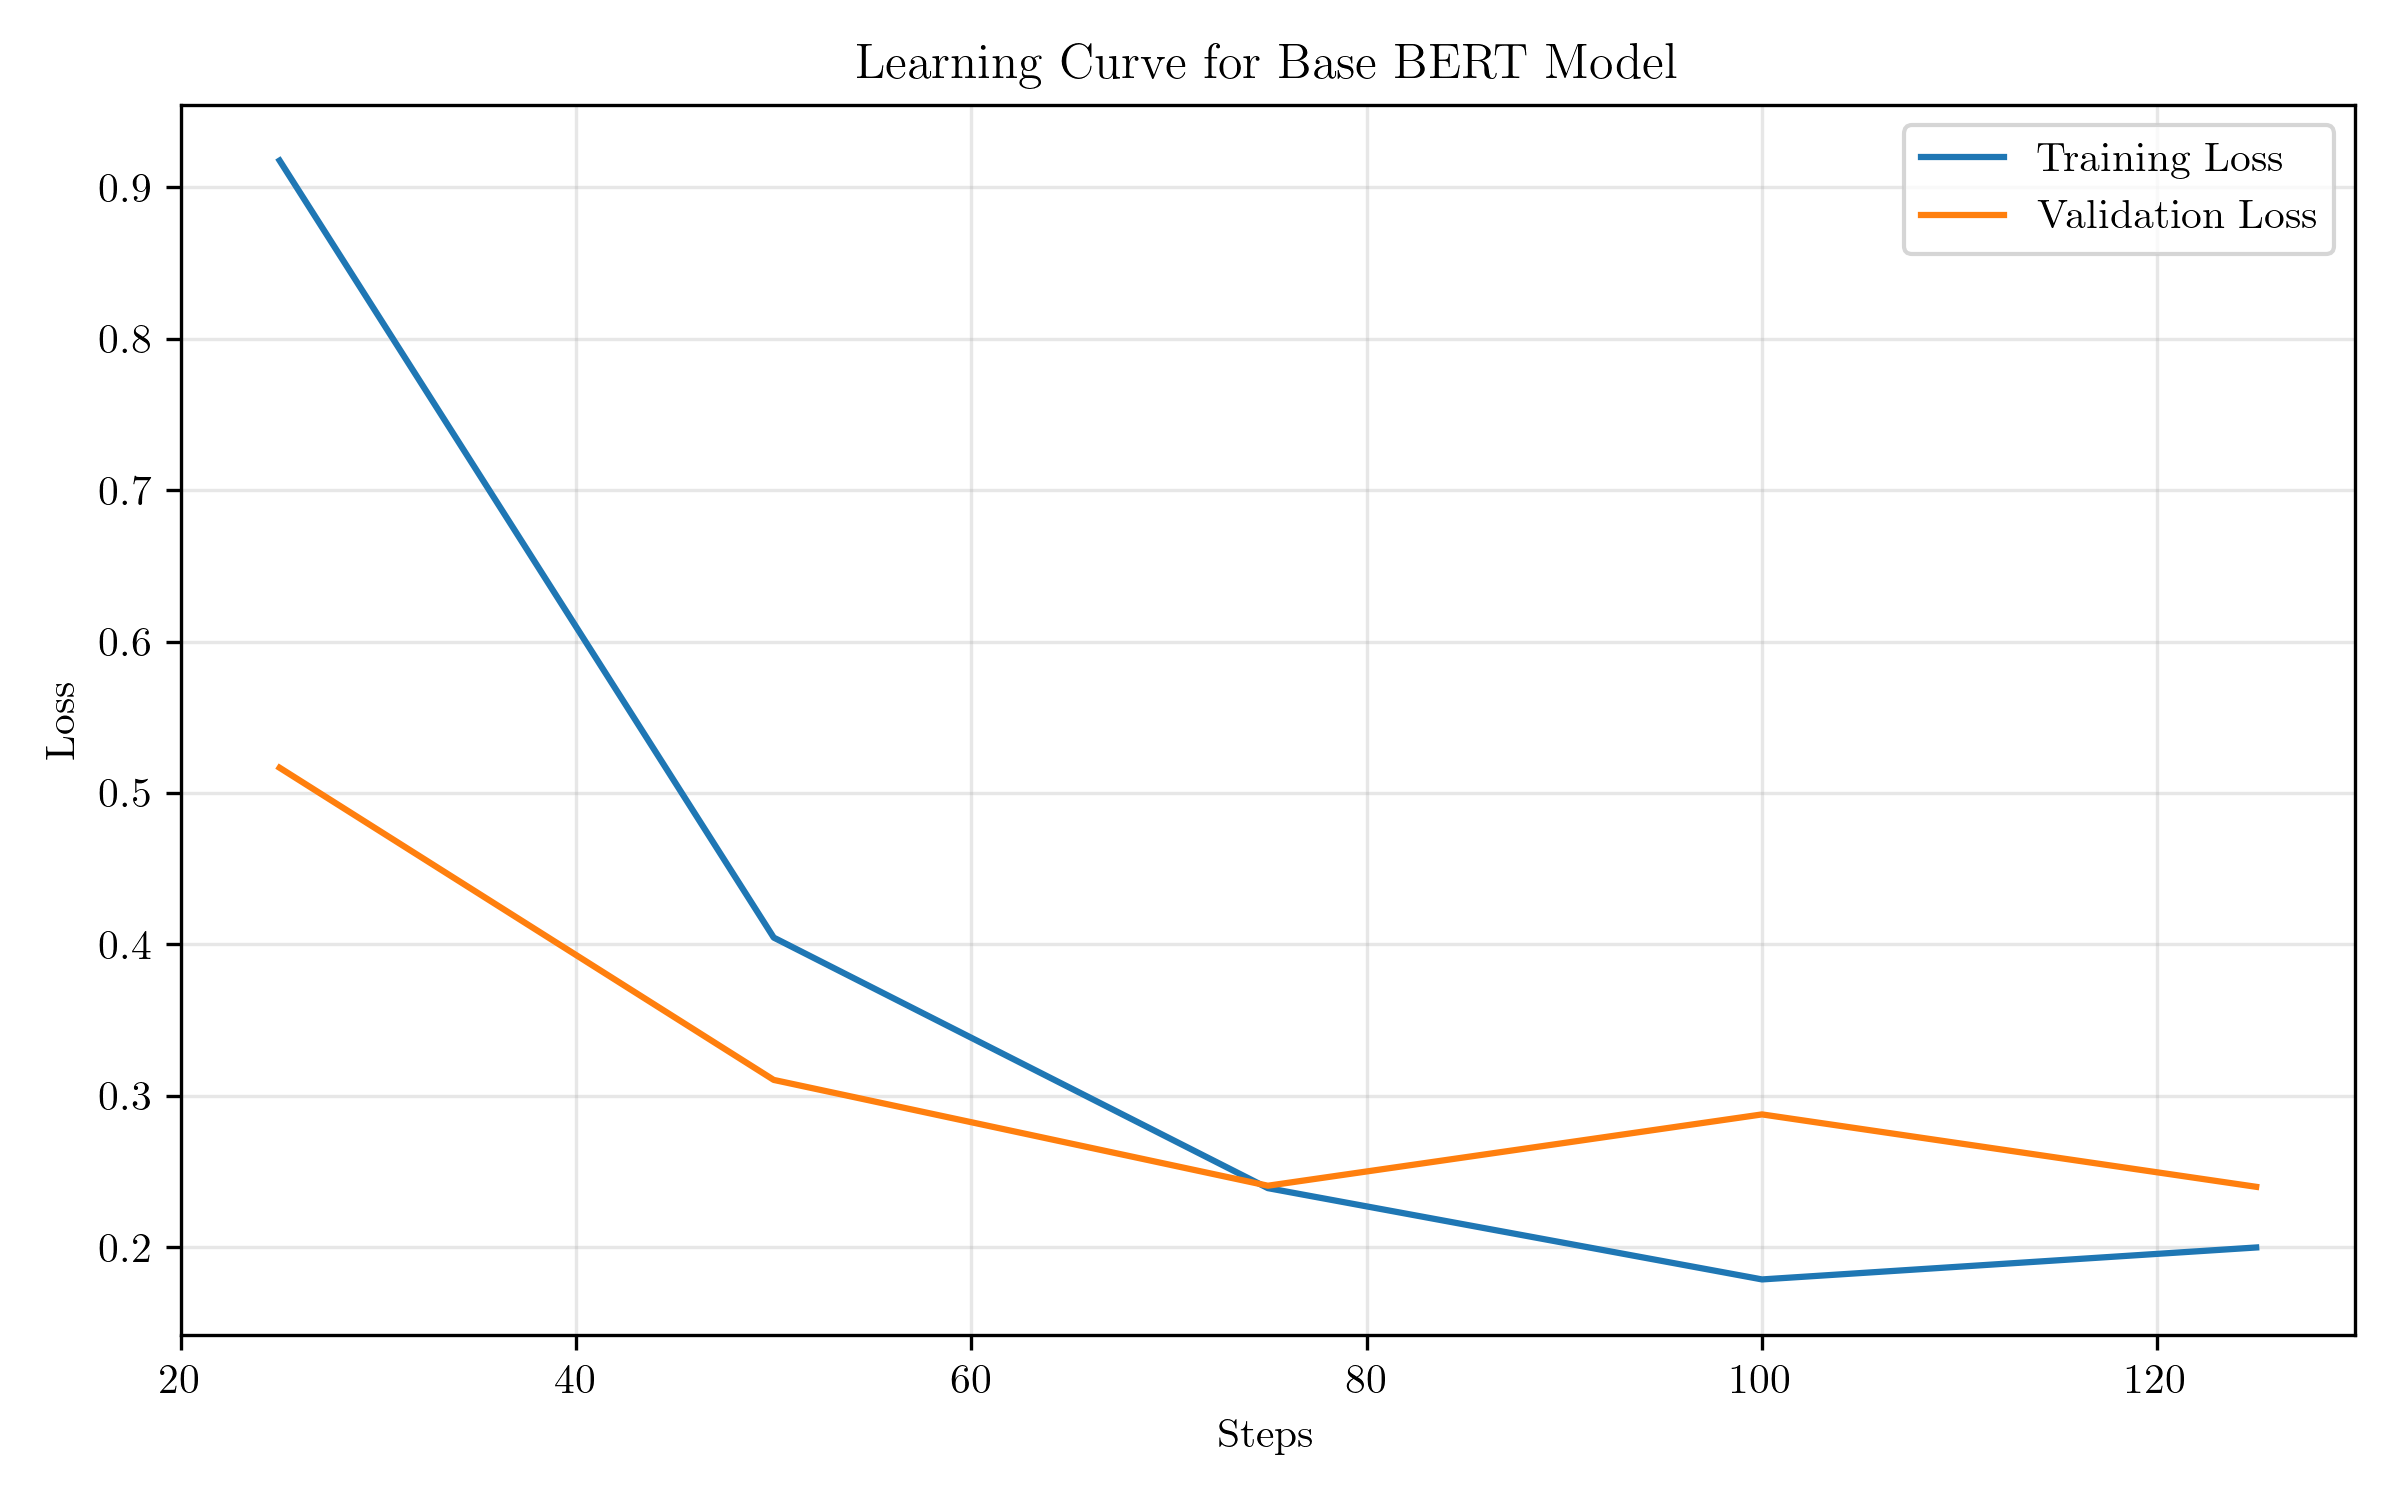
\includegraphics[width=1\linewidth]{assets/base_bert_learning_curve.png}
    \caption{learning curve}
    \label{fig:base_bert_learning_curve}
\end{figure}

\begin{figure}[H]
    \centering
    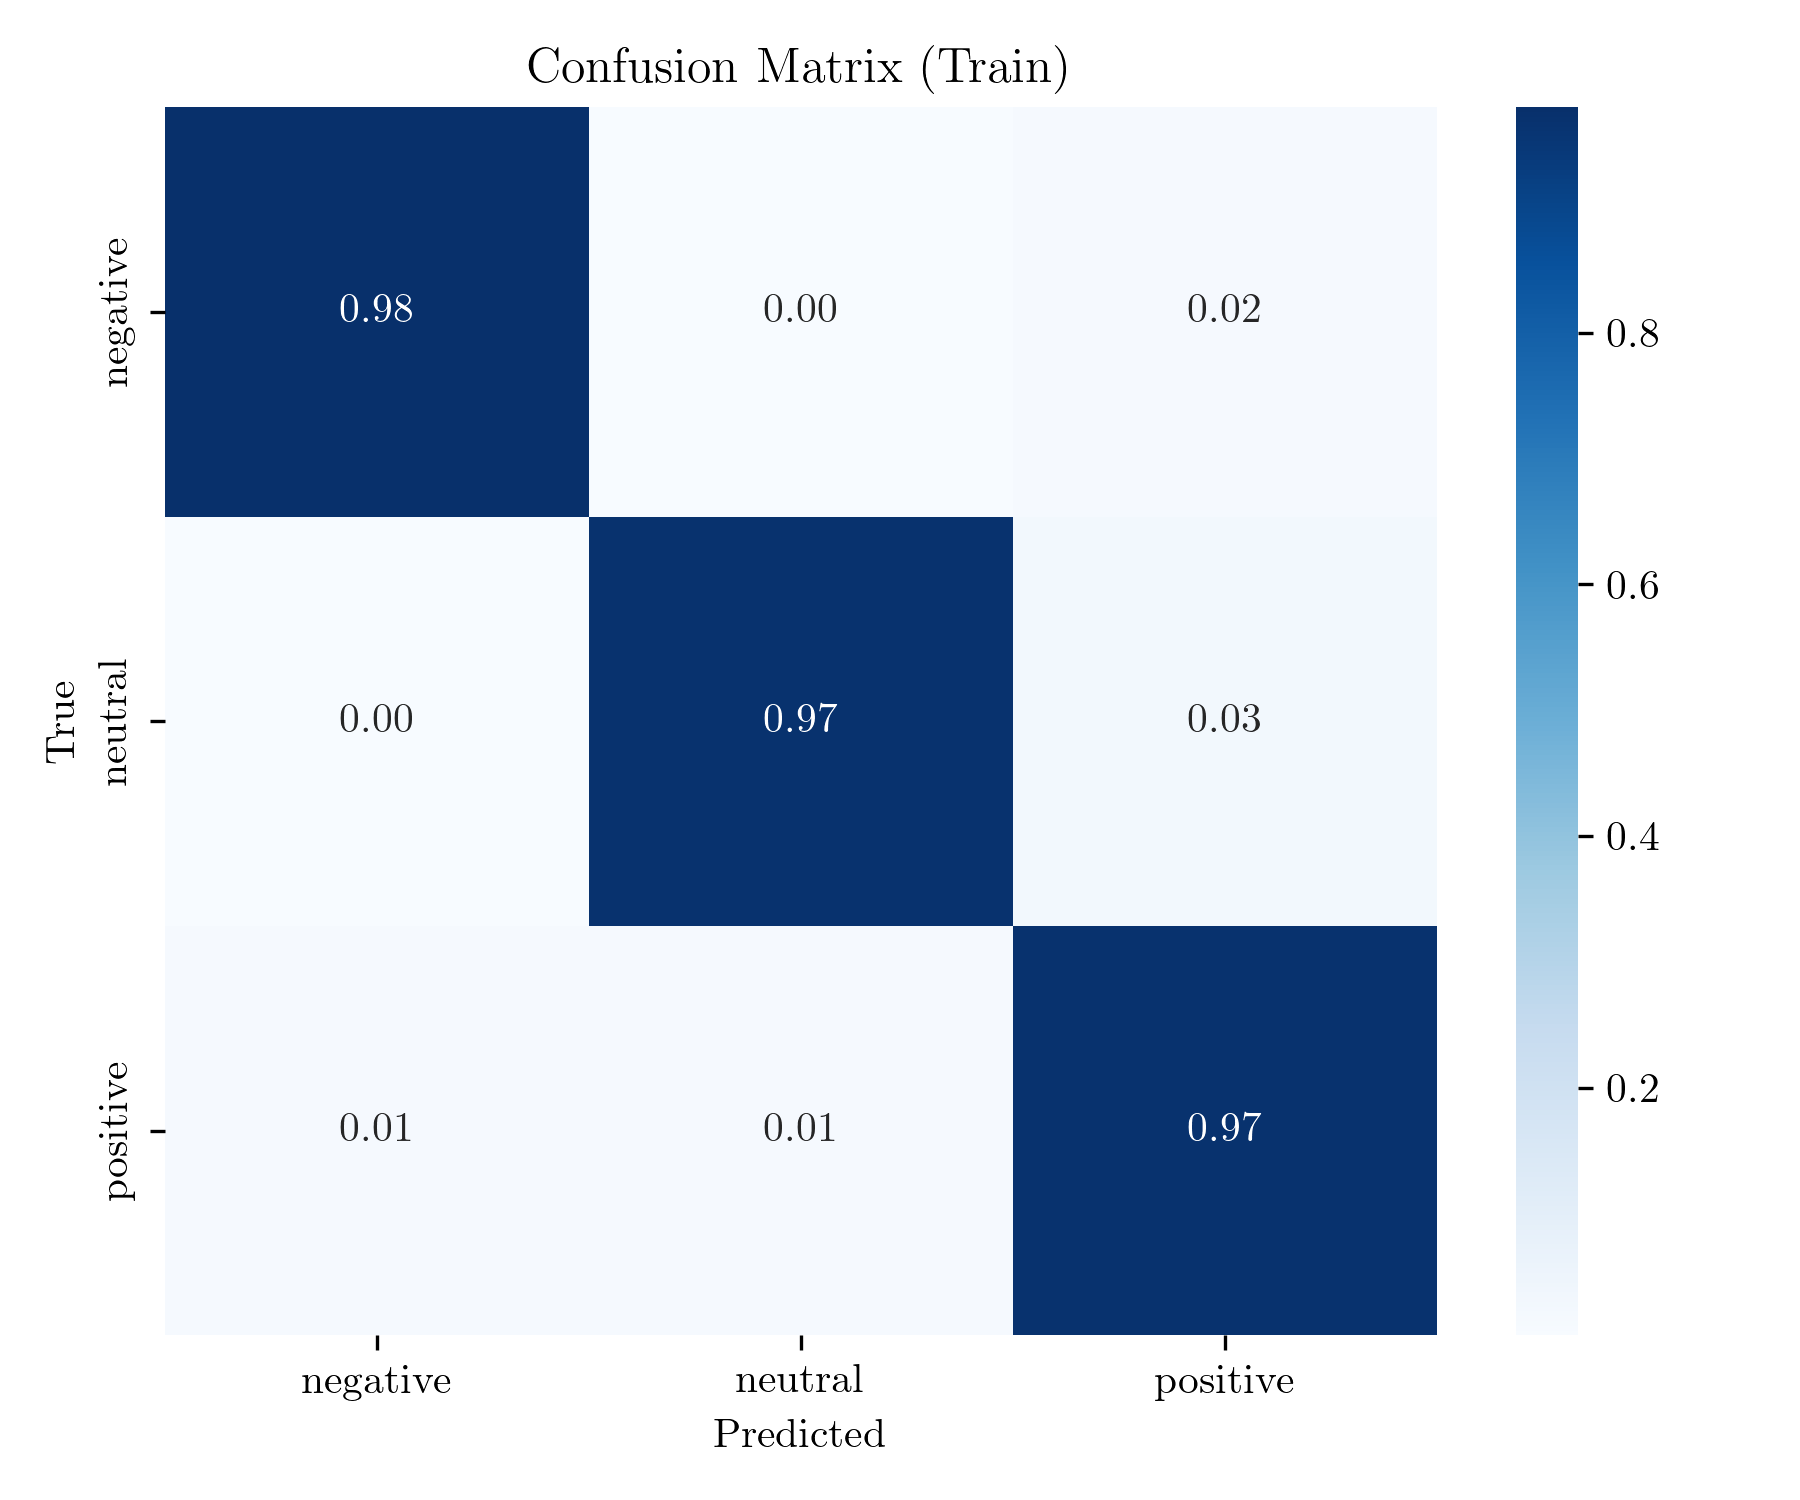
\includegraphics[width=1\linewidth]{assets/base_bert_confusion_matrix_Train.png}
    \caption{base bert conf matri train}
    \label{fig:base_bert_confusion_matrix_Train}
\end{figure}

\begin{table}[H]
\centering
\caption{Classification report for BASE BERT on training data.}
\label{cr_basebert_train}
\begin{tabular}{lcccccc}
\toprule
\textbf{Class} & \textbf{Precision} & \textbf{Recall} & \textbf{F1-Score} & \textbf{Support} \\
\midrule
Negative & 0.98 & 0.98 & 0.98 & 336 \\
Neutral & 0.98 & 0.97 & 0.98 & 336 \\
Positive & 0.96 & 0.97 & 0.96 & 336 \\
\midrule
\textbf{Accuracy} &  &  & 0.97 & 1008 \\
\textbf{Macro avg} & 0.97 & 0.97 & 0.97 & 1008 \\
\textbf{Weighted avg} & 0.97 & 0.97 & 0.97 & 1008 \\
\bottomrule
\end{tabular}
\end{table}

\begin{figure}[H]
    \centering
    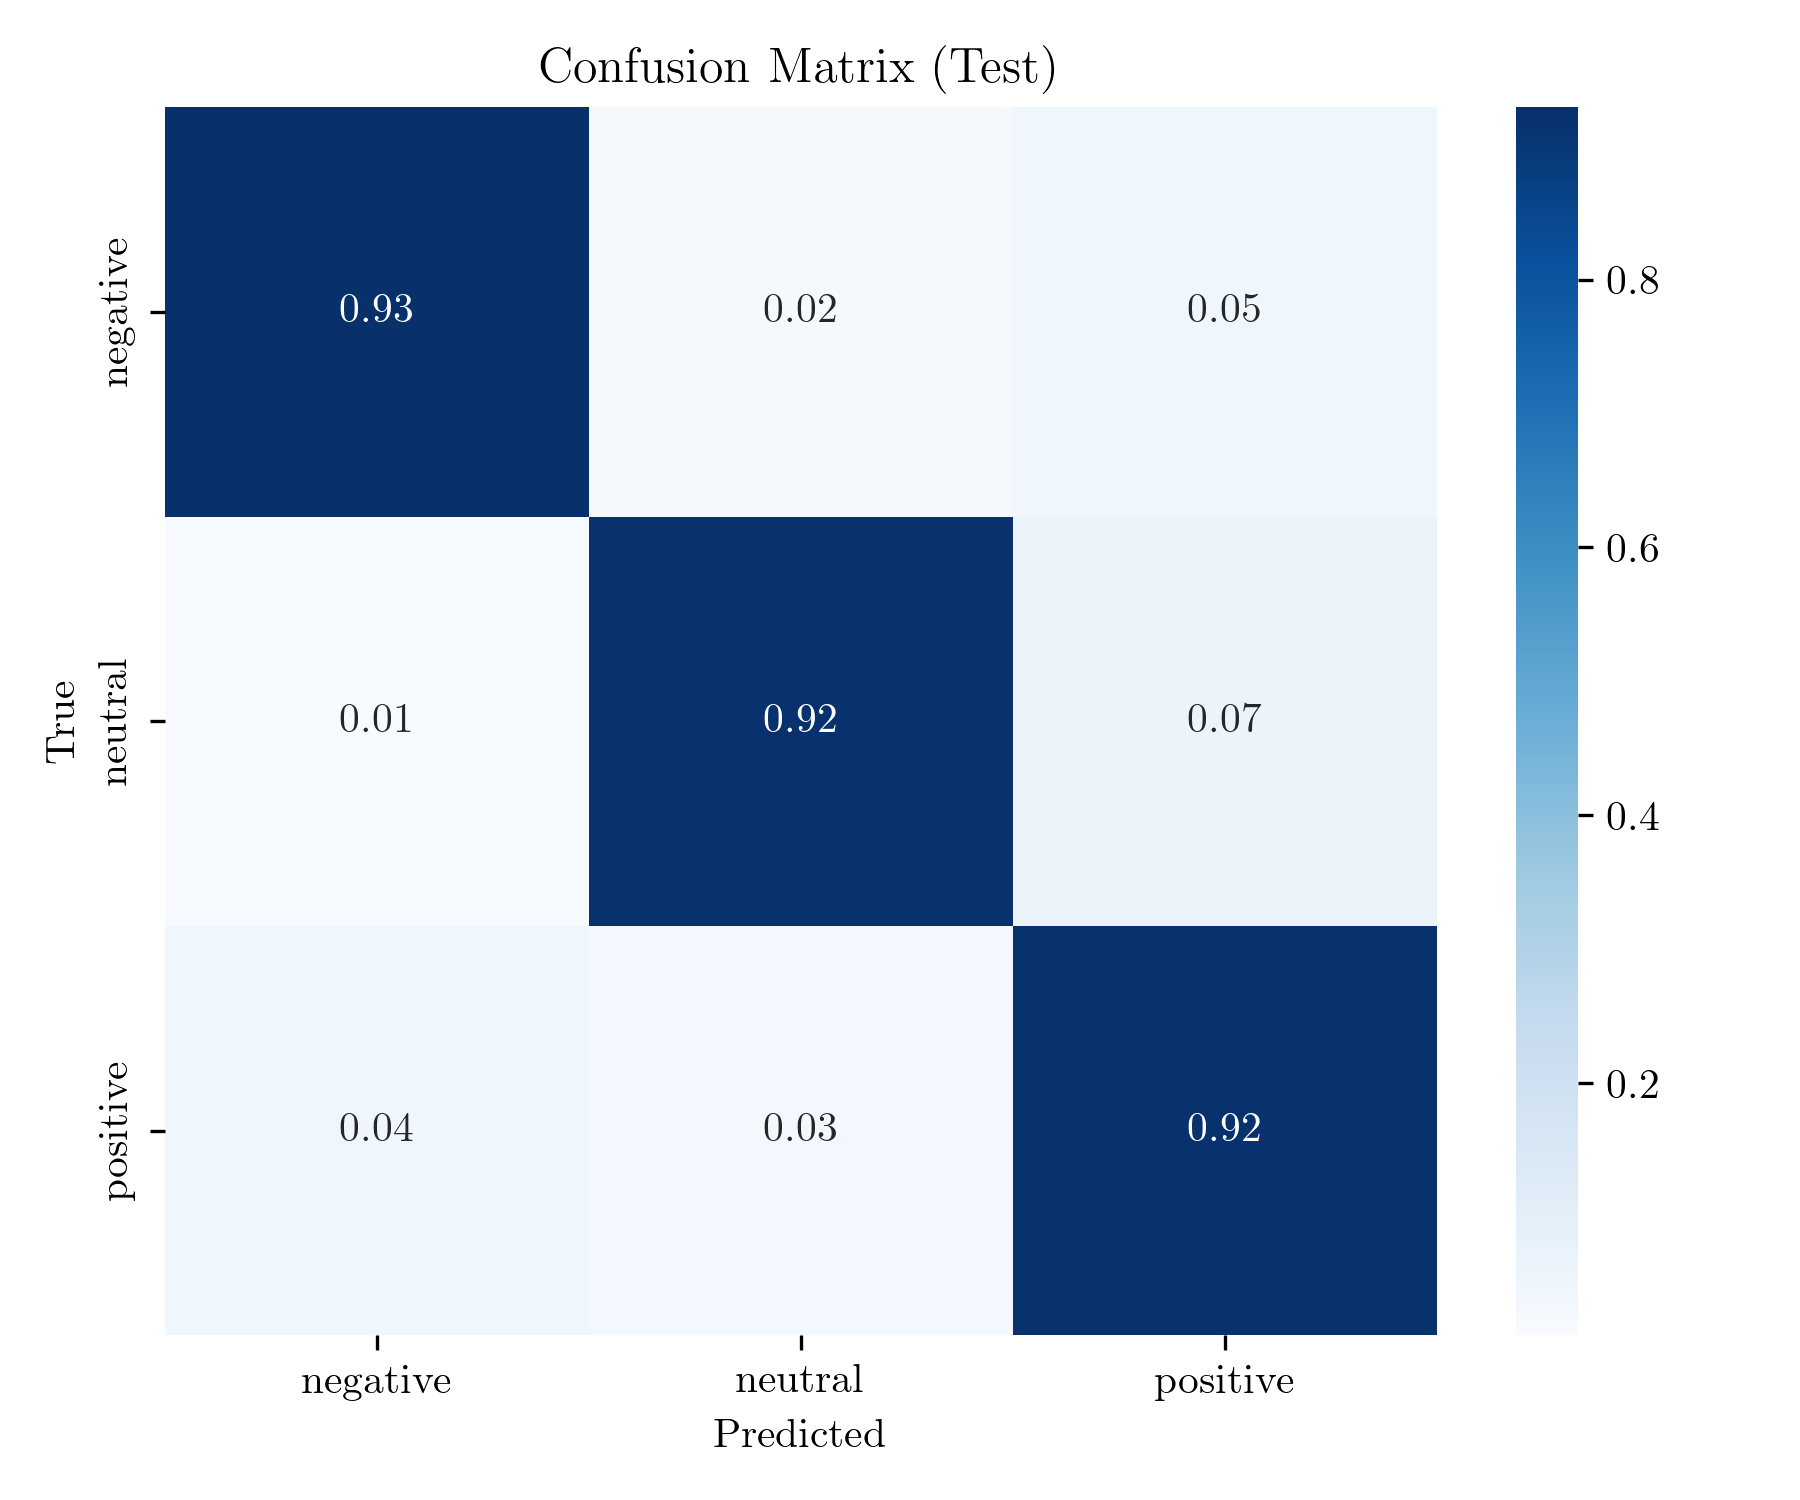
\includegraphics[width=1\linewidth]{assets/base_bert_confusion_matrix_Test.png}
    \caption{base bert cong matrix test}
    \label{fig:base_bert_confusion_matrix_Test}
\end{figure}

\begin{table}[H]
\centering
\caption{Classification report for BASE BERT on test data.}
\label{cr_basebert_test}
\begin{tabular}{lcccccc}
\toprule
\textbf{Class} & \textbf{Precision} & \textbf{Recall} & \textbf{F1-Score} & \textbf{Support} \\
\midrule
Negative & 0.86 & 0.93 & 0.89 & 84 \\
Neutral & 0.98 & 0.92 & 0.95 & 429 \\
Positive & 0.84 & 0.92 & 0.88 & 178 \\
\midrule
\textbf{Accuracy} &  &  & 0.92 & 691 \\
\textbf{Macro avg} & 0.89 & 0.92 & 0.91 & 691 \\
\textbf{Weighted avg} & 0.93 & 0.92 & 0.92 & 691 \\
\bottomrule
\end{tabular}
\end{table}

ligeiro overfitting e tais

\subsection{B. data augmention model}

para esta abordagem foi usada online data augmention nas várias frases do dataset de treino do 75Agree

esta data augmentation consistitiu em:

Back-Translation : Translation-based augmentation using intermediate language pivoting to generate paraphrases.

%em especificio foi traduzir de ingles para uma outra ingles, neste caso o alemão e dps de volta para inglês

Lexical Substitution : Random substitution of words with WordNet-based synonyms.

% big = huge

Template-Based Augmentation : Named Entity-aware augmentation by replacing entities (ORG, DATE, EVENT) using slot-filling over extracted templates.

% Apple, Microsof -> <ORG>, dates -> <DATE>, ...

alguns exemplos desta augmention são

1. In the building and home improvement trade , sales decreased by 22.5 \% to EUR 201.4 mn .

-> in the building and diy trade, sales decreased by 22. 5 \% to eur 201. 4 million.

2. In a media advisory , .......

-> in a media consultation

3. In January-June 2010 , diluted loss per share stood at EUR0 .3 versus EUR0 .1 in the first half of 2009 .

-> in the first half of 2009, diluted loss per share stood atomic number 85 eur0. 3 versus eur0. 1 in the first half of 2009.




\begin{table}[H]
\centering
\caption{Hyperparameter space for ......}
\label{parameters_basebert}
\begin{tabular}{ll}
\toprule
\textbf{Hyperparameter} & \textbf{Possible Values} \\
\midrule
Epochs & $\{1,2,3,4,5\}$ \\
Learning rate & $[10^{-5}, 10^{-2}]$ \\
Weight decay & $[0, 0.5]$ \\
\bottomrule
\end{tabular}
\end{table}

best hyperameters: 

- Num train epochs: 2

- Learning rate: 0.0001

- Weight decay: 0.1

\begin{figure}[H]
    \centering
    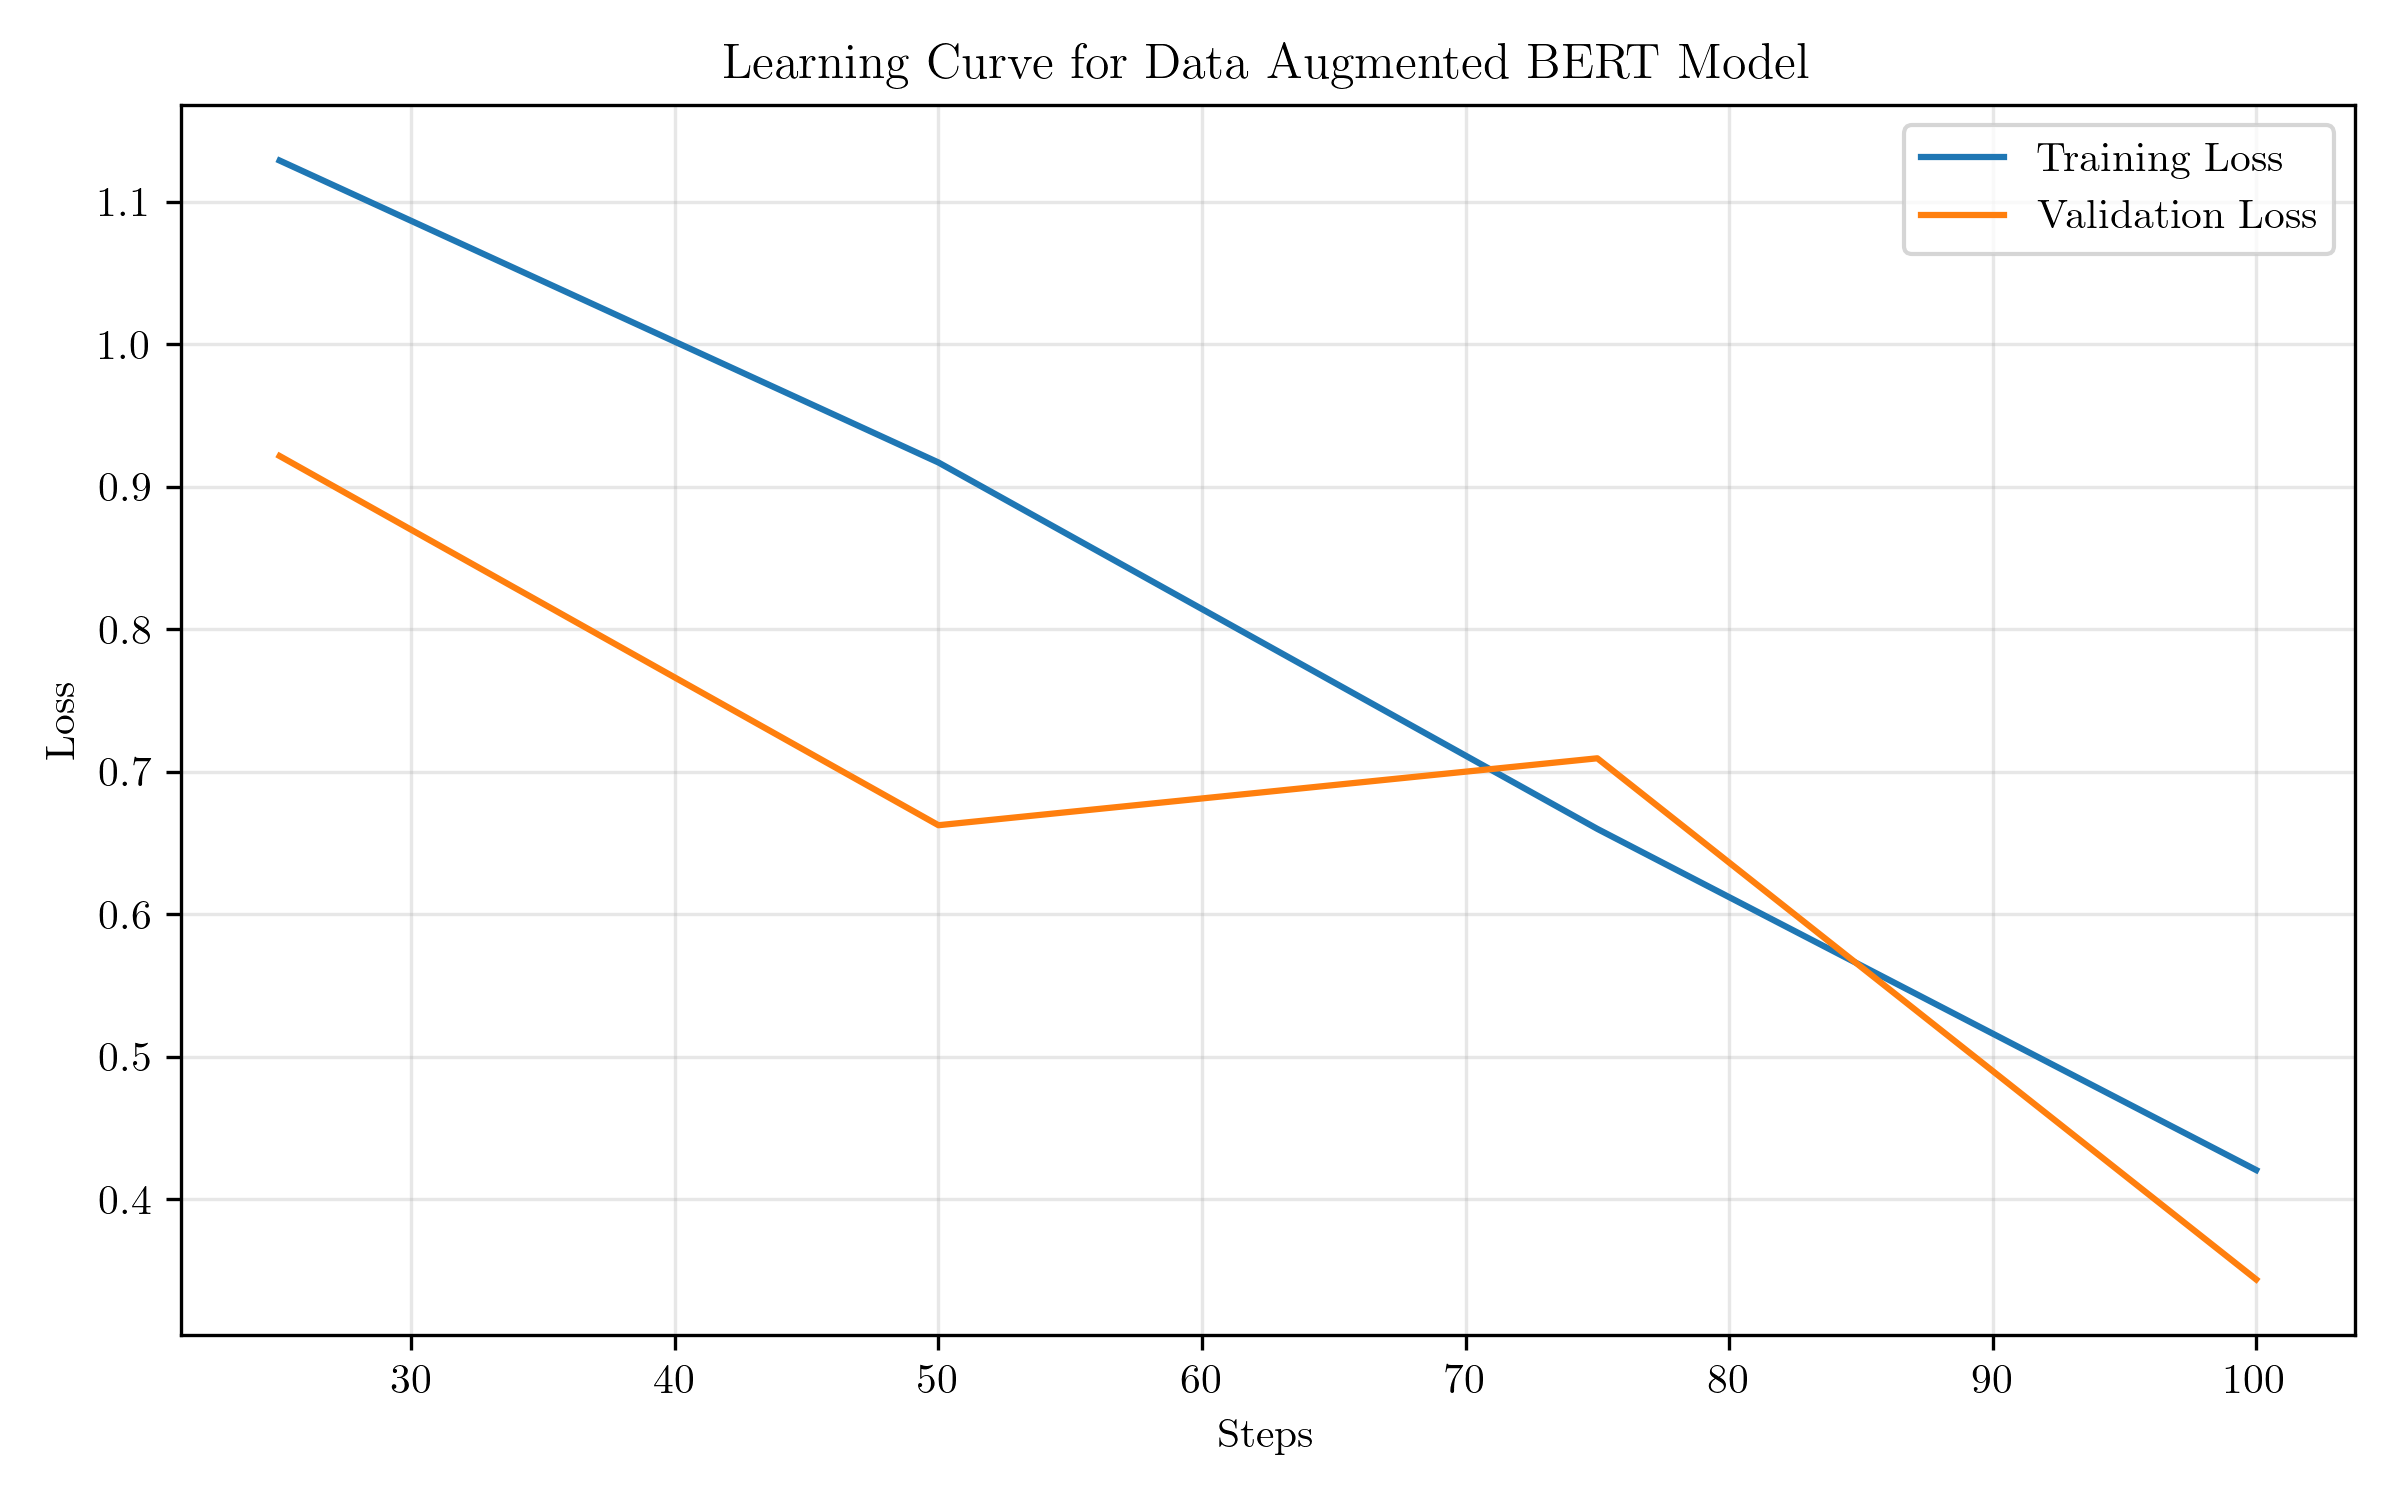
\includegraphics[width=1\linewidth]{assets/data_augmented_bert_learninc_curve.png}
    \caption{learning curve}
    \label{fig:data_augmented_bert_learninc_curve}
\end{figure}

\begin{figure}[H]
    \centering
    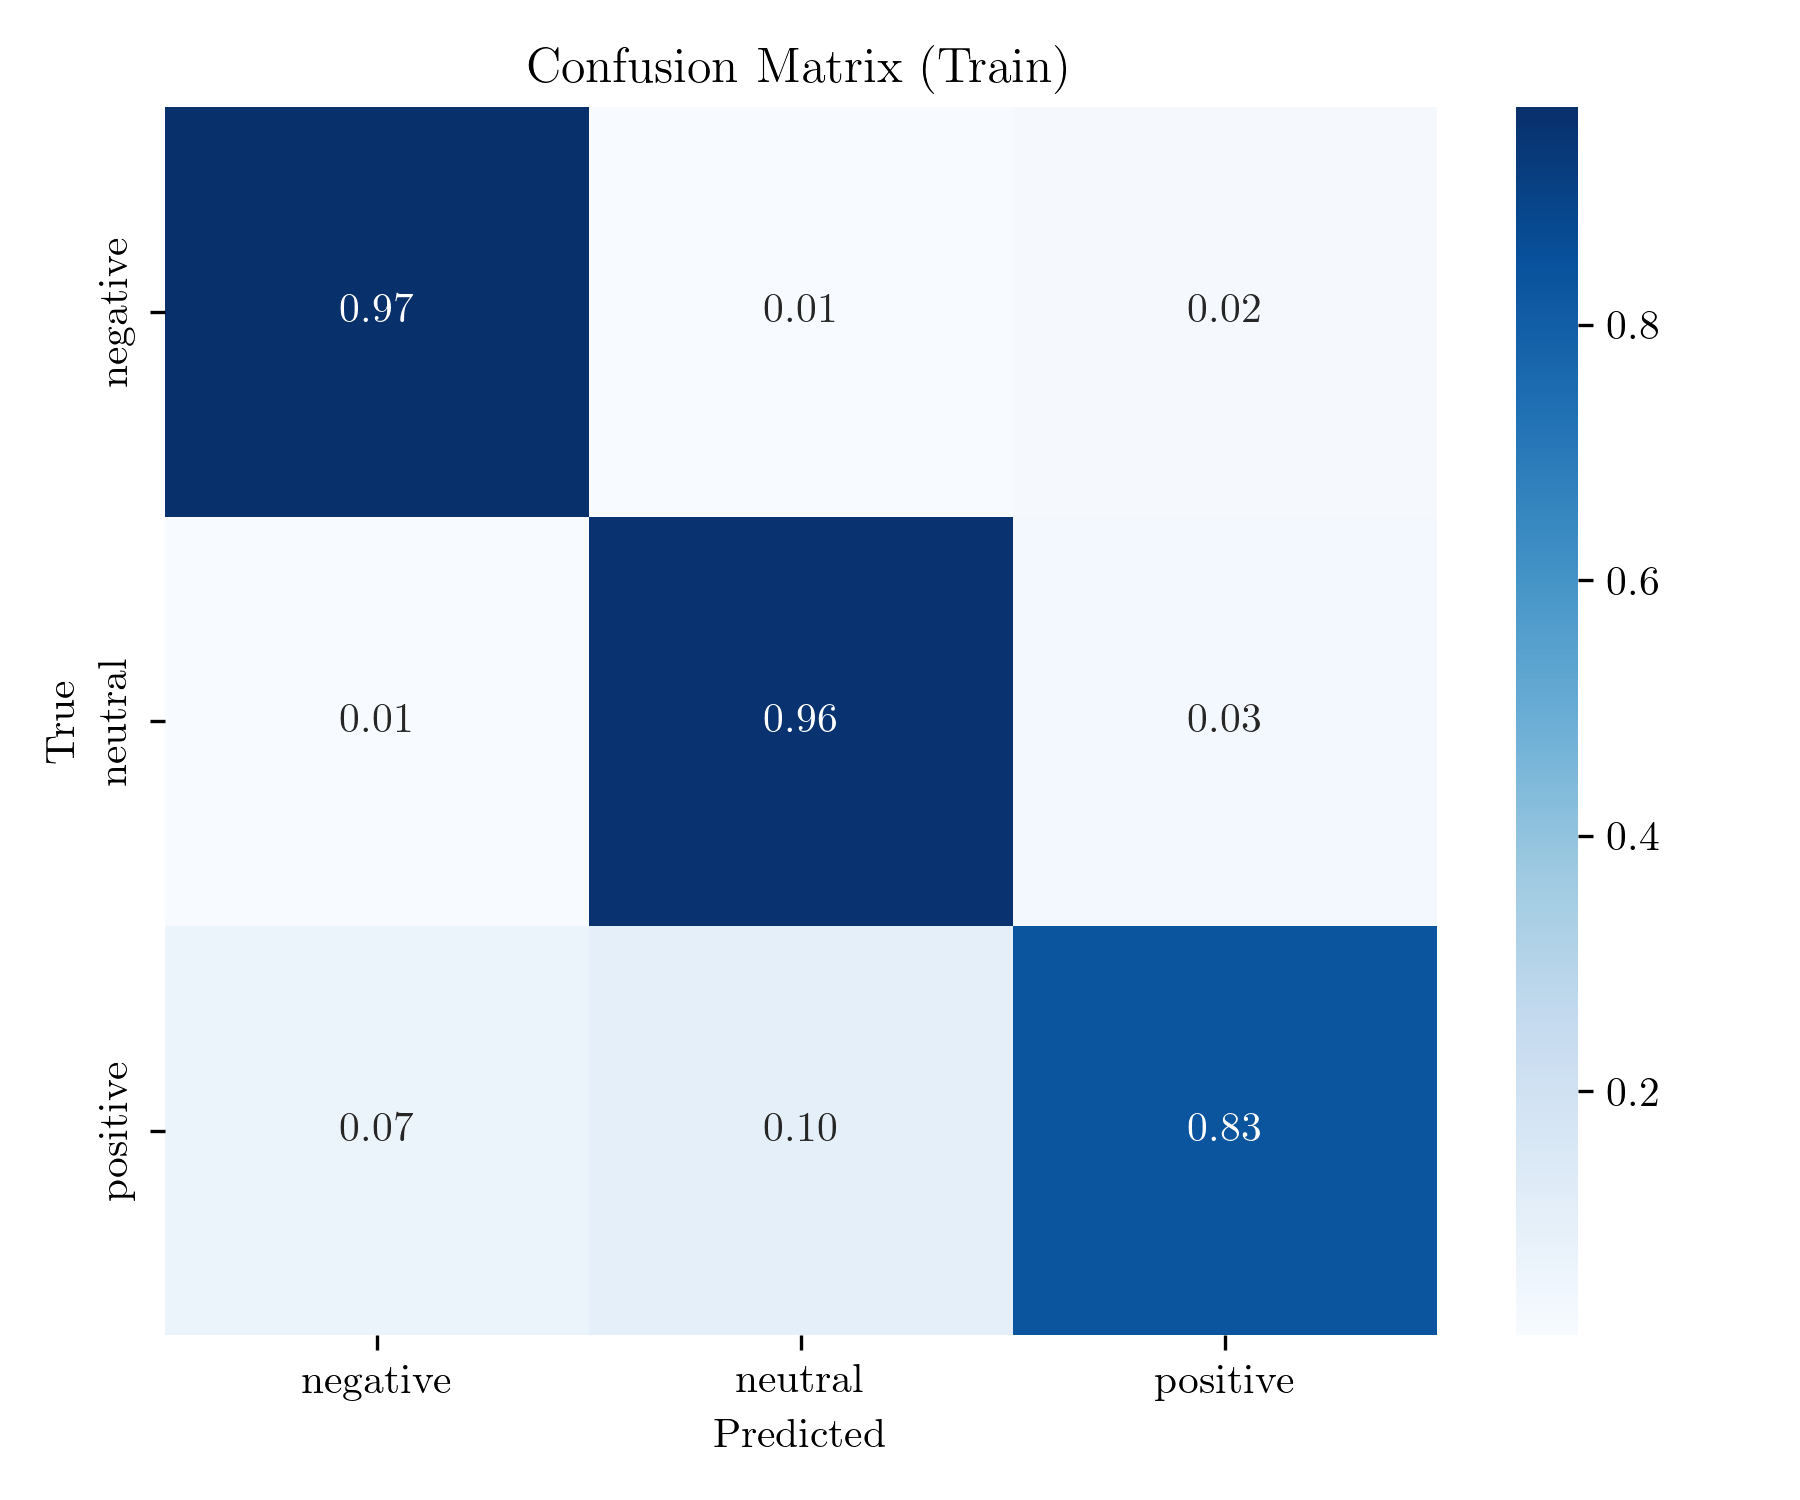
\includegraphics[width=1\linewidth]{assets/dataaugmented_bert_confusion_matrix_Train.png}
    \caption{data augm bert conf matri train}
    \label{fig:dataaugmented_bert_confusion_matrix_Train}
\end{figure}

\begin{table}[H]
\centering
\caption{Classification report for data augm BERT on training data.}
\label{cr_augmbert_train}
\begin{tabular}{lcccccc}
\toprule
\textbf{Class} & \textbf{Precision} & \textbf{Recall} & \textbf{F1-Score} & \textbf{Support} \\
\midrule
Negative & 0.92 & 0.97 & 0.95 & 336 \\
Neutral & 0.90 & 0.96 & 0.93 & 336 \\
Positive & 0.94 & 0.83 & 0.88 & 336 \\
\midrule
\textbf{Accuracy} &  &  & 0.92 & 1008 \\
\textbf{Macro avg} & 0.92 & 0.92 & 0.92 & 1008 \\
\textbf{Weighted avg} & 0.92 & 0.92 & 0.92 & 1008 \\
\bottomrule
\end{tabular}
\end{table}

\begin{figure}[H]
    \centering
    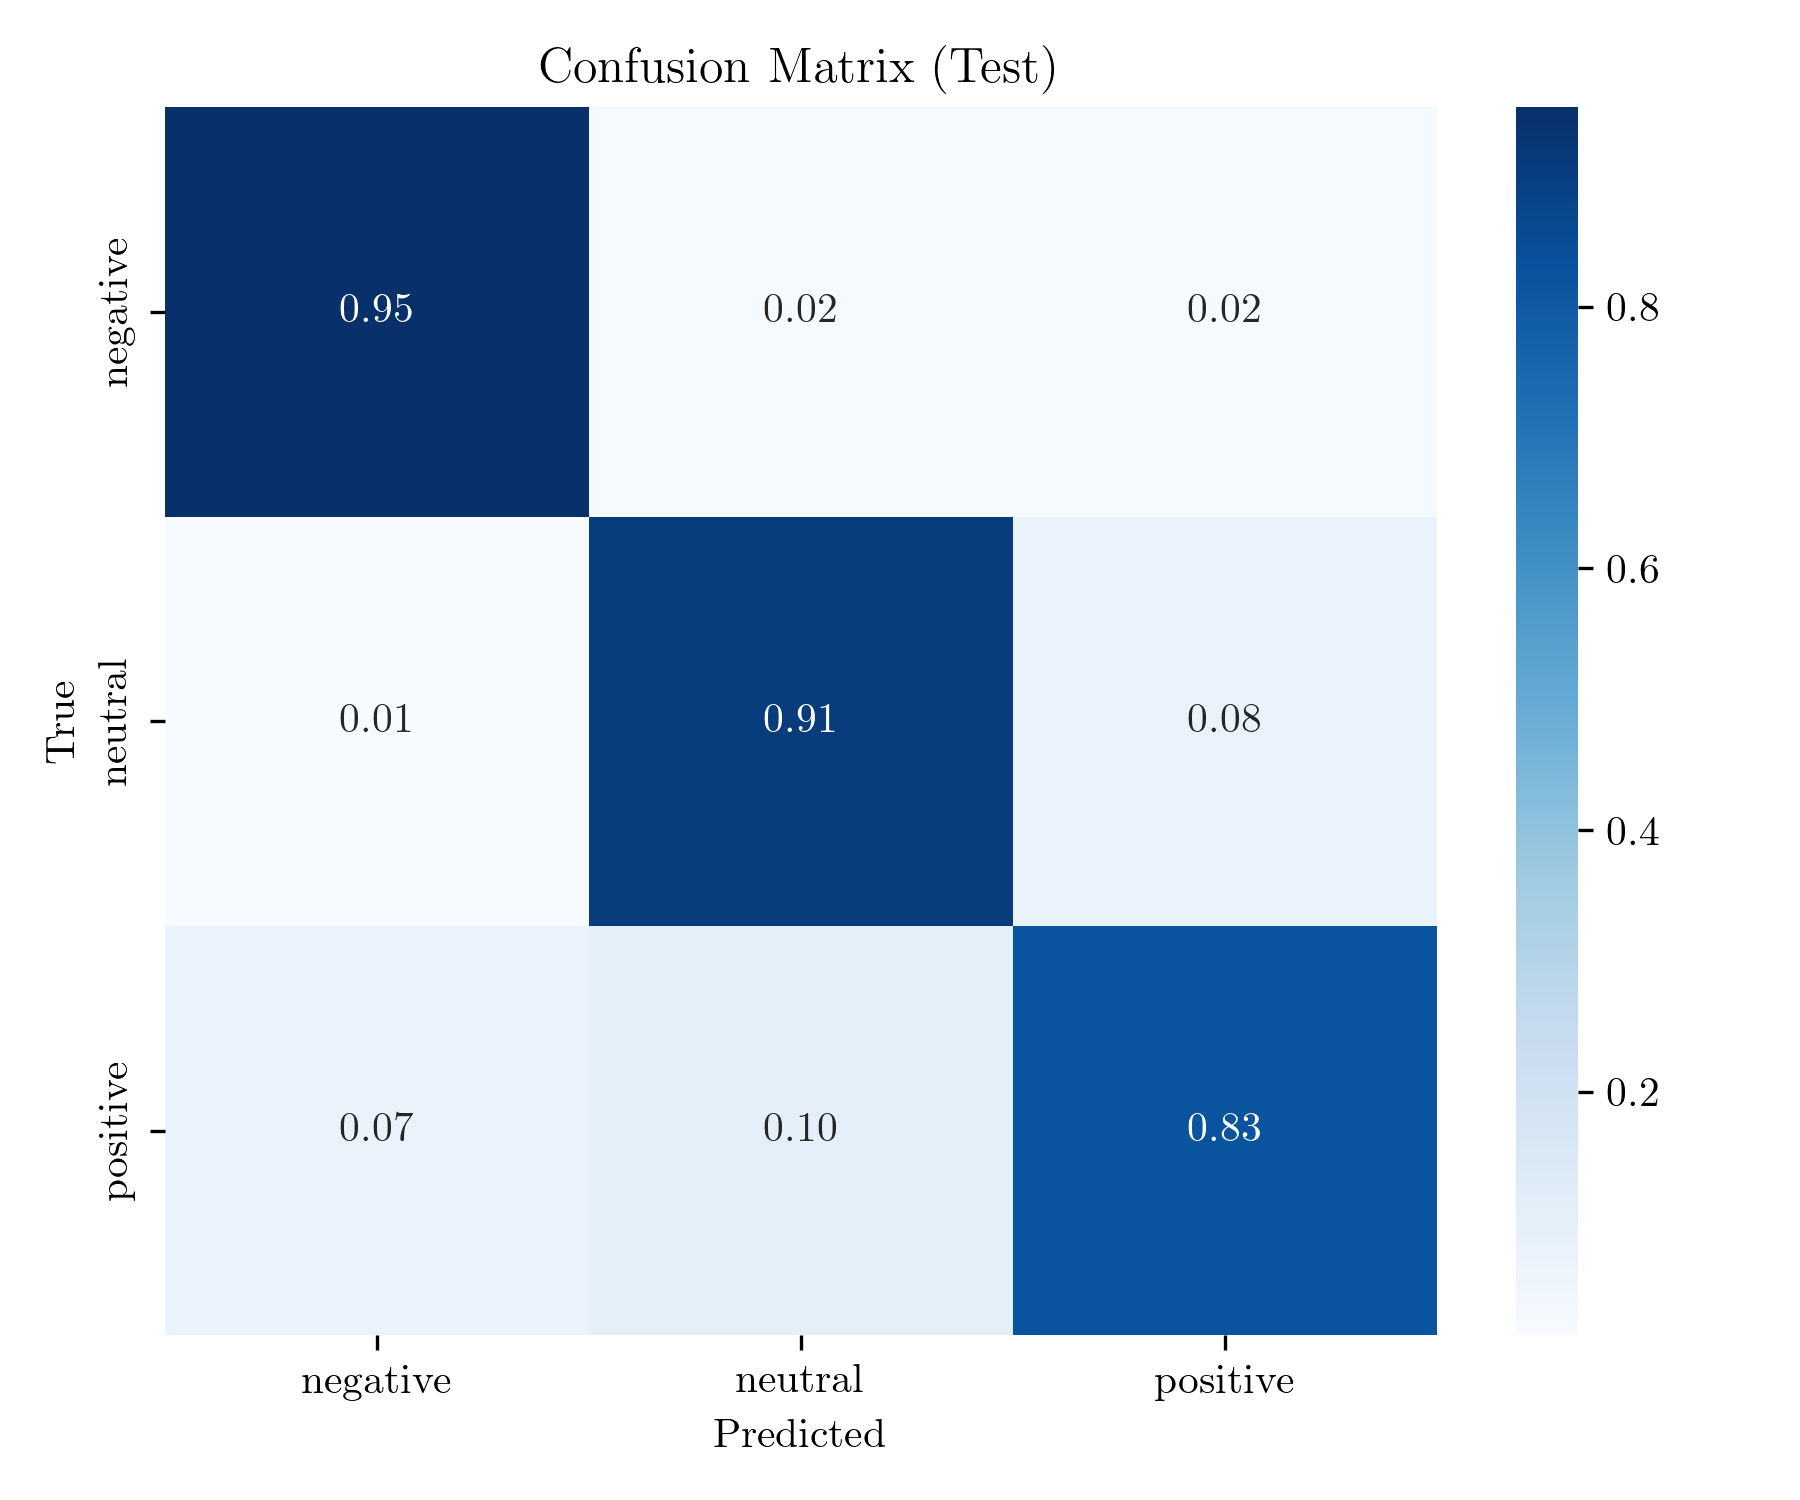
\includegraphics[width=1\linewidth]{assets/dataaugmented_bert_confusion_matrix_Test.png}
    \caption{data augm bert cong matrix test}
    \label{fig:dataaugmented_bert_confusion_matrix_Test}
\end{figure}

\begin{table}[H]
\centering
\caption{Classification report for data augm BERT on test data.}
\label{cr_augmbert_test}
\begin{tabular}{lcccccc}
\toprule
\textbf{Class} & \textbf{Precision} & \textbf{Recall} & \textbf{F1-Score} & \textbf{Support} \\
\midrule
Negative & 0.81 & 0.95 & 0.87 & 84 \\
Neutral & 0.95 & 0.91 & 0.93 & 429 \\
Positive & 0.80 & 0.83 & 0.81 & 178 \\
\midrule
\textbf{Accuracy} &  &  & 0.89 & 691 \\
\textbf{Macro avg} & 0.85 & 0.89 & 0.87 & 691 \\
\textbf{Weighted avg} & 0.90 & 0.89 & 0.89 & 691 \\
\bottomrule
\end{tabular}
\end{table}

os resultados nao apresentam indicios de overfitting e vao ao encontro da literatura

tabela do research, 0.90 de accuracy do finbert q era finetunning do finbert neste dataset ou qq coisa assim



\subsection{weighted model}












\section{Discussion}

results discuttion

eemplo de comparacao

\begin{table}[H]
\centering
\caption{Error metric (MAE) for the fine-tuned models, along with the best performers in the competition.}
\label{tab:model02_results_transposed}
\begin{tabular}{lr}
\toprule
\textbf{Model} & \textbf{MAE (Test Set)} \\
\midrule
Hybrid & 0.8434 \\
Obj. Det. & 1.2645 \\
Inst. Seg. & 1.3415 \\
Team Lacuna (1st) & 0.3299 \\
K\_Junior (2nd) & 0.5698 \\
\bottomrule
\end{tabular}
\end{table}




\section{Conclusion}

conclisao

\begin{figure}[H]
    \centering
    
\includegraphics[width=0.5\linewidth]{image.png}
    \caption{Enter Caption}
    \label{fig:enter-label}
\end{figure}
\section*{Work Load}

Both authors contributed equally to the project.

\bibliographystyle{IEEEtran}
\bibliography{references}

\end{document}



